\chapter{The Solution}

I will discuss the design and implementation of each of the main components of the project separately.

\section{\tsPEG{}}

\subsection{High Level Design}

\tsPEG{} was built using the TypeScript PL. The source code is hosted online at\\
\href{https://github.com/EoinDavey/tsPEG}{github.com/EoinDavey/tsPEG}, and the \tsPEG{} package is available on the NPM package repository at \href{https://www.npmjs.com/package/tspeg}{npmjs.com/package/tspeg}.

\tsPEG{} is self hosting, meaning that the input parser for \tsPEG{} was generated by \tsPEG{}. The software architecture of \tsPEG{} is given in Figure \ref{tspegdiagram}. The usage flow of using \tsPEG{} is as follows. First the user creates a grammar file, specifying the input grammar they want to generate a parser for. The syntax for the grammar file follows a similar pattern to the familiar EBNF syntax for grammar specification. In this file they specify the syntax rules, as well as names of AST fields, and computed properties. The \tsPEG{} binary is then called and it is passed in the grammar file.

\begin{figure}
    \caption{\tsPEG{} High Level Design}
    \label{tspegdiagram}
    \begin{center}
    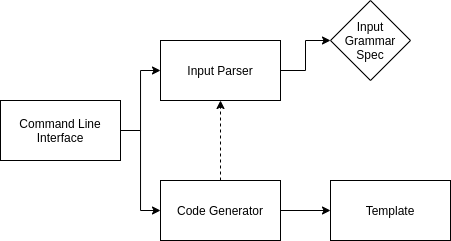
\includegraphics[scale=0.75]{tspegdiagram}
    \end{center}
\end{figure}

\tsPEG{}s own parser consumes the grammar file, and generates an internal description of the grammar. The code generator then takes this grammar specification and generates parsing functions for each rule, as well as TypeScript type declarations and classes for each of the AST nodes. These functions and types are then packaged up into a template file and then written to disk.

\subsection{Grammar specification}

\tsPEG{} uses a custom syntax to define grammars. Figure \ref{tspegexample} contains an example of a grammar specification for simple arithmetic expressions like "1+2*3".

\begin{figure}
    \caption{\tsPEG{} input grammar example}
    \label{tspegexample}
    \begin{lstlisting}
SUM  := head=FAC tail={ op='\+|-' sm=FAC }*
FAC  := head=ATOM tail={ op='\*|/' sm=ATOM }*
ATOM := val=INT
      | '\(' val=SUM '\)'
INT  := val='[0-9]+'
    \end{lstlisting}
\end{figure}

Grammars are defined by a sequence of grammar rules, for example
    \[\text{match} := \text{rule1} \mathbin{|} \text{rule2} \mathbin{|} \text{'a+'}\]
    defines a new rule \verb|match| that tries first \verb|rule1| then \verb|rule2|, then tries to match the regex expression \verb|a+|. The full list of operators is included in Appendix A.

    The \tsPEG{} grammar also allows specification of computed properties, for example Figure \ref{tspegcomputed} defines a rule to match integer literals that stores the value of the integer as a computed property.

\begin{figure}
    \caption{\tsPEG{} computed properties example}
    \label{tspegcomputed}
    \begin{lstlisting}
    INT := literal='[0-9]+'
           .value = number { return parseInt(this.literal) }
    \end{lstlisting}
\end{figure}

\subsection{Bootstrapping}

When developing \tsPEG{}, first a simple input parser was written by hand, supporting only the most basic syntax. A code generator was written that could take in the AST from this simple grammar and output a parser for it. Then the meta-grammar for the input grammar syntax was written and the generator was run. This replaced the hand written parser with a new generated one, self hosting itself and opening itself up to bootstrapping.

This new self hosting generator was then used to add more and more features and operators to itself, eventually resulting in the full self describing meta-grammar for the \tsPEG{} input syntax in Figure \ref{tspegsyntax}.

\begin{figure}
    \caption{\tsPEG{} meta-grammar definition}
    \label{tspegsyntax}
    \begin{lstlisting}
GRAM      := header=HDR? rules=RULEDEF+
HDR       := '---' content='((?!---)(.|\n))*' '---'
RULEDEF   := _ name=NAME _ ':=' _ rule=RULE _
RULE      := head=ALT tail={_ '\|' _ alt=ALT }*
          .list = ALT[] { return [this.head, ...this.tail.map((x) => x.alt)]; }
ALT       := matches=MATCHSPEC+ attrs=ATTR*
MATCHSPEC := _ named={name=NAME _ '=' _}? rule=POSTOP _
POSTOP    := pre=PREOP op='\+|\*|\?'?
            .optional = boolean { return this.op !== null && this.op === '?'}
PREOP     := op='\&|!'? at=ATOM
ATOM      := name=NAME !'\s*:='
           | match=STRLIT
           | '{' _ sub=RULE _ '}'
ATTR      := _ '.' name=NAME _ '=' _ type='[^\s\{]+' _ '\{'
    action='([^\{\}\\]|(\\.))*'
'\}'
NAME      := '[a-zA-Z_]+'
STRLIT    := '\'' val='([^\'\\]|(\\.))*' '\''
_         := '\s*'
    \end{lstlisting}
\end{figure}
